\documentclass{ctexart}
\begin{document}
\title{计算物理作业 14}
\author{刘畅, PB09203226}
\maketitle

{\bf [作业 14]:} 在二维正方网格上, 按 HPP 模型的规则, 模拟一圈环形
压缩波的传播过程, 作出不同时间的图形.

\section{算法}
HPP 模型是一种元胞自动机, 每一时刻用一个4位二进制数表示格点某个位置四个方向
有无粒子进入这个格点. 演化规则为:
\begin{center}
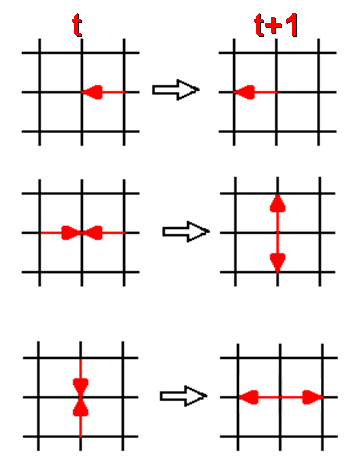
\includegraphics[width=2in]{hpp.png}
\end{center}
第一个规则对应粒子的传播, 后两个规则对应粒子的散射. 这三个过程都是动量守恒和粒子数
守恒的.

在下面编程的过程中还需要考虑的是格点边界上的演化规则. 书上没有写, 所以我规定
粒子碰到边界后, 如果是穿过边界的, 就反射回来. 这样按照上面的规则就可以来写程序了.

\section{程序}
首先我们要确定的是格点在计算机内存中如何表示, 和前面类似, 也是用一个二维数组:
\begin{verbatim}
char (*lattice)[dim] = (char (*)[dim])
    malloc(dim * dim * sizeof(char));
\end{verbatim}
考虑到这个二维数组可能比较大, 栈空间不够, 因此要在堆上分配.

格点的每一个元素是一个 \verb|char| 型整数, 最低的4位用来表示上下左右四个方向
有没有粒子进入. 有就为1, 没有就为0. 为了代码清楚起见, 需要下面几个宏来方便地从
\verb|char| 型整数中提取出这些信息.
\begin{verbatim}
/* macros for packing and unpacking directional information */
#define get_incoming(x, k)      ((x) & (1 << (k)))
#define set_incoming(x, k)      ((x) |= (1 << (k)))
#define unset_incoming(x, k)    ((x) &= ~(1 << (k)))
\end{verbatim}
如果你对位运算不太熟悉参见 {\sl C: A Reference Manual}, Fifth Edition, Samuel
P.~Harbison III, Guy L.~Steele Jr. 除此之外, 为避免幻数的出现, 定义下面
的枚举类型来表示4个方向:
\begin{verbatim}
/* 0th bit of an int indicates particle content
 * coming from the left
 * 1th -- right, 2 -- up, 3 -- down
 * NDIR -- number of total directions
 */
enum { LEFT, RIGHT, UP, DOWN, NDIR };
\end{verbatim}

接下来编写模拟 HPP 规则的例程, 我们把它叫做 \verb|take_next_step()|,
模拟的每一步都调用这个函数来使得自动机向前演化. 这个例程需要旧的格点和新的格点
的指针, 他们对应的空间由调用者分配. 这例程主要的工作是按照规则更新格点:
\begin{verbatim}
for (i = 0; i < dim; i++) {
    for (j = 0; j < dim; j++) {
        char incoming[NDIR];
        int k;
        for (k = 0; k < NDIR; k++)
            incoming[k] = get_incoming(oldlat[i][j], k);
        /* rules for HPP model: */
        /* \rightattow\leftarrow  =>  \uparrow\downarrow */
        if (incoming[LEFT] && incoming[RIGHT]
            && i != 0 && i != dim-1) {
            set_incoming(newlat[i-1][j], DOWN);
            set_incoming(newlat[i+1][j], UP);
            unset_incoming(oldlat[i][j], LEFT);
            unset_incoming(oldlat[i][j], RIGHT);
            incoming[LEFT] = 0;
            incoming[RIGHT] = 0;
        }
        /* \downarrow\uparrow => \leftarrow\rightarrow */
        if (incoming[UP] && incoming[DOWN]
            && j != 0 && j != dim-1) {
            set_incoming(newlat[i][j-1], RIGHT);
            set_incoming(newlat[i][j+1], LEFT);
            unset_incoming(oldlat[i][j], UP);
            unset_incoming(oldlat[i][j], DOWN);
            incoming[UP] = 0;
            incoming[DOWN] = 0;
        }
        /* rules 1: particles pass right through */
        if (incoming[LEFT] && !incoming[RIGHT]
            && j != dim-1) {
            set_incoming(newlat[i][j+1], LEFT);
            unset_incoming(oldlat[i][j], LEFT);
            incoming[LEFT] = 0;
        }
        if (incoming[RIGHT] && !incoming[LEFT]
            && j != 0) {
            set_incoming(newlat[i][j-1], RIGHT);
            unset_incoming(oldlat[i][j], RIGHT);
            incoming[RIGHT] = 0;
        }
        if (incoming[UP] && !incoming[DOWN]
            && i != dim-1) {
            set_incoming(newlat[i-1][j], UP);
            unset_incoming(oldlat[i][j], UP);
            incoming[UP] = 0;
        }
        if (incoming[DOWN] && !incoming[UP]
            && i != 0) {
            set_incoming(newlat[i+1][j], DOWN);
            unset_incoming(oldlat[i][j], DOWN);
            incoming[DOWN] = 0;
        }
        /* boundary rules -- reflection at boundary */
        if (j == 0 && incoming[RIGHT]) {
            set_incoming(newlat[i][j], LEFT);
            unset_incoming(oldlat[i][j], RIGHT);
        }
        if (j == dim-1 && incoming[LEFT]) {
            set_incoming(newlat[i][j], RIGHT);
            unset_incoming(oldlat[i][j], LEFT);
        }
        if (i == 0 && incoming[DOWN]) {
            set_incoming(newlat[i][j], UP);
            unset_incoming(oldlat[i][j], DOWN);
        }
        if (i == dim-1 && incoming[UP]) {
            set_incoming(newlat[i][j], DOWN);
            unset_incoming(oldlat[i][j], UP);
        }
    }
}
\end{verbatim}
这段代码就是把上面算法一节中的规则翻译成 C 语言, 首先处理粒子碰撞的情形,
然后处理粒子传播的情形, 最后处理边界.

现在就可以来编写HPP 模拟的例程了, 函数名叫 \verb|hpp_simulation()|.
这个例程首先在堆上分配两个格点, 一个旧的一个新的, 用来传给 \verb|take_next_step()|.
然后初始化旧的格点:
\begin{verbatim}
/* initialize the lattice */
double radius, angle;
memset(oldlat, 0, dim * dim * sizeof(char));
memset(newlat, 0, dim * dim * sizeof(char));
for (radius = r0; radius < r1; radius += 0.5) {
    for (angle = 0; angle < 2*CONST_PI; angle += 0.5/radius) {
        int direc = conv_angle_to_direc(angle);
        int x = radius * cos(angle) + dim/2;
        int y = radius * sin(angle) + dim/2;
        set_incoming(oldlat[y][x], direc);
    }
}
\end{verbatim}
\verb|conv_angle_to_direc| 按照某个格点在极坐标中的角度设置其位置的粒子的
初始方向, 在这个程序中我们把初始方向设置为指向格点中心:
\begin{verbatim}
/* convert angle to direction
 *     U
 *   L   R
 *     D
 */
int conv_angle_to_direc(double angle)
{
    if (angle > CONST_PI / 4 && angle < CONST_PI * 3 / 4)
        return UP;
    if (angle >= CONST_PI * 3 / 4 && angle < CONST_PI * 5 / 4)
        return LEFT;
    if (angle >= CONST_PI * 5 / 4 && angle < CONST_PI * 7 / 4)
        return DOWN;
    return RIGHT;
}
\end{verbatim}

接下来就可以做实际的模拟了:
\begin{verbatim}
/* do the simulation */
int i;
char (*tmp)[dim];
for (i = 0; i < nsteps; i++) {
    take_next_step((char *) oldlat, (char *) newlat, dim);
    /* swap oldlat and newlat */
    tmp = oldlat;
    oldlat = newlat;
    newlat = tmp;
}
\end{verbatim}
上面的代码通过交换指针的方式避免了拷贝整个格点这一缓慢的操作, 除此之外没有什么好
解释的, 就是迭代 \verb|nsteps| 步调用 \verb|take_next_step()|.

\verb|main.c| 的其余部分是上面几个函数的单元测试, 不是非常重要, 就不解释了.

\section{模拟结果}
下面是模拟 \verb|nsteps| 的结果, 其中 \verb|nsteps| 依次取下面的值:
(见 \verb|main.c|)
\[
2^n,\quad n=0,\ldots, 5;\qquad
40+10n,\quad n=0,\ldots, 15
\]
初始的构形为粒子在一个圆环上向内运动. 从模拟结果可以看到有明显的波动现象.
\input res_plot

\end{document}